\chapter{引言}
\label{chap:introduction}

\begin{figure}[htb]
    \centering
    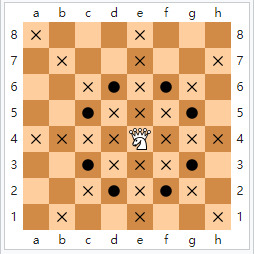
\includegraphics[width=0.4\textwidth]{amazon.PNG}
    \caption[超级皇后]{%
      超级皇后走法,可以像皇后与骑士一样移动%
      \cite{wikiAmazon}。}
    \label{fig:superQueen}
  \end{figure}

\section{游戏背景与规则}
国际象棋影响深远受众广泛,在经历了漫长的传播与演变后形成了今日的规则。
A History of Chess 详细记载了其演变过程与各种游戏规则的变种与分支\cite{murray2015history}。在中世纪之后的很长一段时间内,皇后棋子(或者被称为Amazon)可以像现代皇后或骑士一样移动,只不过由于太过强力,相对平衡的现代皇后在国际象棋规则中作为正统胜出。
指导老师与笔者受其启发,构思出一款国际象棋衍生游戏—超级皇后对战。
规则描述如下:指定大小的棋盘(8x8,12x12等)有黑白两个超级皇后;超级皇后的落子规则可指定(皇后走法,骑士走法,混合走法),不可越位,不可攻击对方;每当超级皇后离开当前位置,该位置变为不可落子的死地;胜利条件为封死对方超级皇后的行动。

\begin{figure}[htb]
    \centering
    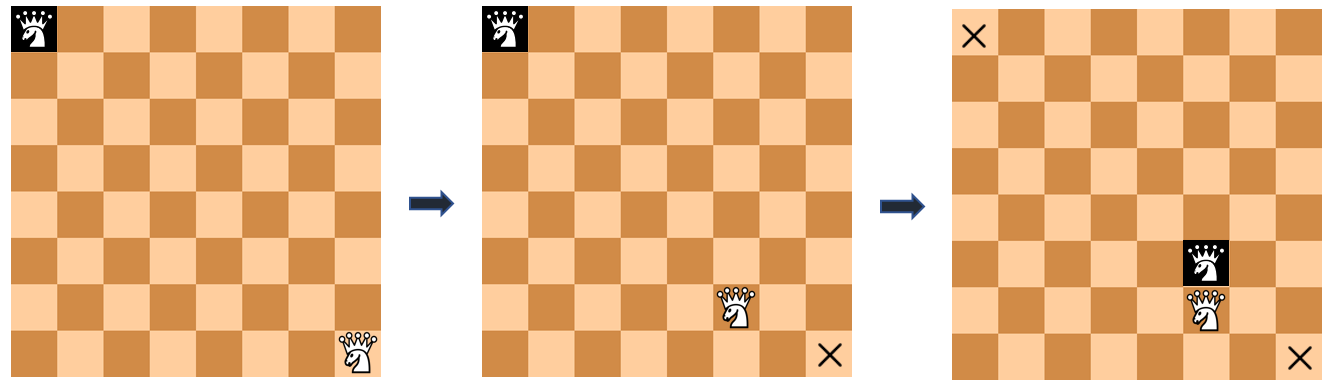
\includegraphics[width=0.4\textwidth]{rules.PNG}
    \caption[游戏规则]{%
      超级皇后对战游戏规则%
      }
    \label{fig:superQueenRules}
  \end{figure}


\section{本文工作}

\section{论文结构}

% \cite{Book:GV1996}
% \cite{wikiAmazon}